% Provenance (never printed): see sources/outline_sources.md (Year 2: Goldschmidt's
% classification; the chondritic Earth; core, mantle and crust compositions; trace
% elements and normalised diagrams). Curves from figdata/bachelor-2/geochem.py; exercise
% and problem values in the Book 4 scratch calculator calc/ch03.py.
\chapter{العناصر في الأرض}\label{ch:b2:elements-in-the-earth}

يحوي طنّ من صخور القارات نحو مليغرام ونصف من
الذهب. أمّا طنّ من الكوندريتات الكربونية التي عرضها الفصل السابق، وهي أكثر الأحجار
التي تسقط من السماء بدائيةً، فيحوي نحو مئة ضعف ذلك. وقد تجمّعت
الأرض من مثل هذه المادة، فالذهب ليس مفقودًا من
الأرض: إنه في مكان آخر. فإذا جمعنا التراكيب المقدّرة للنواة وللأرض
السيليكاتية مع كتلة النواة، تبيّن أن أكثر من 99 في المئة من
ذهب الأرض موجود في النواة، حيث غاص مع الحديد في مطلع
تاريخ الأرض. والذهب واحد من عائلة من العناصر تتبع الحديد
الفلزي؛ وعناصر أخرى تتبع الكبريتيد، وأخرى الصخر السيليكاتي، وأخرى أيضًا تفلت
إلى الهواء. يفرز هذا الفصل العناصر في هذه العائلات، ويستعمل
الكوندريتات لإعادة بناء تركيب الأرض كلها ولوزن
نواتها، ويصف تراكيب الوشاح والقشرة المحيطية والقشرة
القارية، ويقدّم العناصر النزرة والمخطّطات التي يقرأ عليها
الجيوكيميائيون تاريخ الصخر.
% ledger: rg03:ucc-trace, lodders:ci-table, mcd03:core, ms95:pm-trace, data:prem

\begin{recall}
للأرض نواة فلزية، معظمها من الحديد، تحت وشاح سيليكاتي وقشرة
رقيقة؛ ويعطي علم الزلازل نصف قطر كل طبقة وكثافتها، والنواة
أقل كثافة بنسبة 5 إلى 10 في المئة مما يكون عليه الحديد النقي عند الضغط ودرجة الحرارة
نفسيهما، وهذا يستدعي وجود عناصر خفيفة فيها: والمرشّحة هي السيليكون والكبريت والكربون
والأكسجين والهيدروجين (مجلد السنة الأولى).
وتقيس الكهرسلبية لعنصرٍ شدّةَ جذب ذرّاته
لإلكترونات الرابطة، ويتوقّف نصف قطر الأيون على شحنته وعلى
عدد جيرانه (مجلد السنة الأولى من كتب الكيمياء). ومعامل
التوزيع هو نسبة تركيزي مادة في طورين في
توازن (مجلد السنة الأولى من كتب الكيمياء). وقد قُدّمت الكوندريتات والكوندريتات
الكربونية \omterm{def:b2:planet-formation-meteorites:condensation}{وتسلسل التكاثف} في
\cref{ch:b2:planet-formation-meteorites}.
\end{recall}
% ledger: badro:core

\section{تصنيف غولدشميت}

حين ينصهر جسم كوندريتي تنفصل مادته إلى سوائل لا تمتزج: فلز
كثيف من الحديد والنيكل، وسائل كبريتيدي إن كان الكبريت كافيًا،
ومصهور سيليكاتي، وفوقها طور غازي. ويتوزّع كل عنصر بين
هذه الأطوار حسب كيميائه، ويُرى التوزيع نفسه في
صهر الخامات، حيث ينفصل في الفرن الحديد المنصهر والمطفأة الكبريتيدية والخَبَث
السيليكاتي.

\begin{definition}[تصنيف غولدشميت]
\label{def:b2:elements-in-the-earth:goldschmidt}
\emph{تصنيف غولدشميت}\index{تصنيف غولدشميت} يفرز
العناصر حسب الطور الذي تفضّله في جسم ينفصل إلى فلز
وكبريتيد وسيليكات وغاز. ف\emph{العنصر المحبّ للصخور}\index{العنصر المحبّ للصخور}
يفضّل السيليكات والأكاسيد؛ و\emph{العنصر المحبّ للحديد}\index{العنصر المحبّ للحديد}
يفضّل الحديد الفلزي؛ و\emph{العنصر المحبّ
للكبريتيد}\index{العنصر المحبّ للكبريتيد} يفضّل الكبريتيد؛ و\emph{العنصر المحبّ
للغلاف الجوي}\index{العنصر المحبّ للغلاف الجوي} يبقى في الغاز، غازًا أو مركّبًا
متطايرًا.
\end{definition}

تتبع هذه الأصناف كيمياء الترابط. فالعناصر المحبّة للصخور، مثل الفلزات
القلوية والقلوية الترابية والألومنيوم والتيتانيوم \omterm{def:b2:elements-in-the-earth:ree}{والعناصر الأرضية النادرة}، تتخلّى
عن إلكتروناتها بسهولة للأكسجين، الأعلى منها كهرسلبيةً بكثير،
وتكوّن معه روابط أيونية. والعناصر المحبّة للحديد، أي فلزات مجموعة البلاتين والذهب
والنيكل والكوبالت، كهرسلبيتها قريبة من كهرسلبية الحديد، وترتبط ضعيفًا
بالأكسجين وتذوب في الفلز. والعناصر المحبّة للكبريتيد، ومنها النحاس والزنك والرصاص
والفضة والكادميوم، تكوّن مع الكبريت روابط أكثر تساهمية.
والعناصر المحبّة للغلاف الجوي هي الغازات النبيلة والنيتروجين والهيدروجين. وكثير من
العناصر ينتمي إلى صنفين، حسب الظروف: فالحديد نفسه
محبّ للحديد في جسم غني بالفلز ومحبّ للصخور في الوشاح المؤكسَد، حيث
يقيم في الأوليفين والبيروكسين؛ والتنغستن والموليبدنوم محبّان للحديد في
الأرض، لكن جزءًا كبيرًا منهما بقي في الوشاح (الشكل أدناه).

\begin{omfigure}
\centering
\begin{tikzpicture}[x=0.62cm, y=-0.62cm,
  lith/.style={fill=brown!30}, sid/.style={fill=blue!30!gray!45},
  chal/.style={fill=orange!45}, atm/.style={fill=cyan!15}, none/.style={fill=black!8},
  cell/.style={draw=black!55, minimum size=0.58cm, inner sep=0pt, font=\scriptsize}]
\foreach \s/\c/\r/\k in {H/1/1/atm, He/18/1/atm,
  Li/1/2/lith, Be/2/2/lith, B/13/2/lith, C/14/2/atm, N/15/2/atm, O/16/2/lith,
  F/17/2/lith, Ne/18/2/atm,
  Na/1/3/lith, Mg/2/3/lith, Al/13/3/lith, Si/14/3/lith, P/15/3/lith, S/16/3/chal,
  Cl/17/3/lith, Ar/18/3/atm,
  K/1/4/lith, Ca/2/4/lith, Sc/3/4/lith, Ti/4/4/lith, V/5/4/lith, Cr/6/4/lith,
  Mn/7/4/lith, Fe/8/4/sid, Co/9/4/sid, Ni/10/4/sid, Cu/11/4/chal, Zn/12/4/chal,
  Ga/13/4/chal, Ge/14/4/sid, As/15/4/chal, Se/16/4/chal, Br/17/4/lith, Kr/18/4/atm,
  Rb/1/5/lith, Sr/2/5/lith, Y/3/5/lith, Zr/4/5/lith, Nb/5/5/lith, Mo/6/5/sid,
  Tc/7/5/none, Ru/8/5/sid, Rh/9/5/sid, Pd/10/5/sid, Ag/11/5/chal, Cd/12/5/chal,
  In/13/5/chal, Sn/14/5/chal, Sb/15/5/chal, Te/16/5/chal, I/17/5/lith, Xe/18/5/atm,
  Cs/1/6/lith, Ba/2/6/lith, Hf/4/6/lith, Ta/5/6/lith, W/6/6/sid, Re/7/6/sid,
  Os/8/6/sid, Ir/9/6/sid, Pt/10/6/sid, Au/11/6/sid, Hg/12/6/chal, Tl/13/6/chal,
  Pb/14/6/chal, Bi/15/6/chal, Po/16/6/none, At/17/6/none, Rn/18/6/none,
  La/3/8/lith, Ce/4/8/lith, Pr/5/8/lith, Nd/6/8/lith, Pm/7/8/none, Sm/8/8/lith,
  Eu/9/8/lith, Gd/10/8/lith, Tb/11/8/lith, Dy/12/8/lith, Ho/13/8/lith,
  Er/14/8/lith, Tm/15/8/lith, Yb/16/8/lith, Lu/17/8/lith,
  Th/4/9/lith, U/6/9/lith}
  \node[cell, \k] at (\c,\r) {\s};
\node[cell, lith, minimum width=0.58cm] at (3,6) {\tiny La--Lu};
\draw[black!50, -latex] (3,6.32) -- (3,7.65);
% legend
\foreach \k/\t/\x/\y in {lith/{محبّ للصخور}/3.6/1, sid/{محبّ للحديد}/3.6/2,
  chal/{محبّ للكبريتيد}/3.6/3, atm/{محبّ للغلاف الجوي}/7.8/1, none/{لا نظير مستقرًا له}/7.8/2}
  \node[cell, \k, label={[font=\scriptsize]east:\t}] at (\x,\y) {};
\end{tikzpicture}
\par\smallskip{\small أصناف غولدشميت للعناصر المستقرة وللثوريوم واليورانيوم، اللذين بقيت نظائرهما الطويلة العمر منذ ولادة الأرض، ملوّنة حسب الصنف
الغالب في الأرض؛ وعناصر صفّ الأتربة النادرة موضوعة في الخانة
La--Lu. وعدة عناصر تنتمي إلى صنفين: فالحديد والنيكل والكوبالت أيضًا
محبّة للصخور في الوشاح المؤكسَد؛ والكربون أيضًا محبّ للحديد، والفوسفور
محبّ للحديد في النيازك.}
\end{omfigure}

\section{الأرض الكوندريتية}

لا يستطيع أحد أخذ عيّنة من الأرض كلها: فالنواة بعيدة المنال، والوشاح
لا يبلغ السطح إلا قطعًا. ولذلك يُبنى تركيب الأرض الكلية
من دليلين: النيازك، التي هي عيّنات من المادة
التي تكوّنت منها الكواكب، وصخور الوشاح والمصاهير
الآتية منه.

\begin{definition}[كوندريت CI]\label{def:b2:elements-in-the-earth:ci}
\emph{كوندريت CI}\index{كوندريت CI} عضو في مجموعة من
الكوندريتات الكربونية سُمّيت باسم نيزك إيفونا: أحجار سوداء هشّة
مكوّنة كلها تقريبًا من أرضية دقيقة الحبيبات، غنية بالمعادن الحاملة للماء وبالكربون،
تكاد تخلو من \omterm{def:b2:planet-formation-meteorites:chondrule}{الكوندرولات}. وباستثناء الهيدروجين والكربون والنيتروجين والأكسجين
والغازات النبيلة، فإن تركيبها هو الأقرب بين كل المواد المعروفة إلى تركيب
الفوتوسفير الشمسي؛ وهي التركيب المرجعي في الجيوكيمياء.
\end{definition}

تضمّ المجموعة خمسة نيازك، كلها سقطات: ألايس (1806)، وأورغاي
(1864)، وتونك (1911)، وإيفونا (1938)، وريفلستوك (1965)؛ وأورغاي أكبرها،
بأربعة عشر كيلوغرامًا. والتركيب المعتمد للمجموعة متوسط مرجّح
لتحاليلها، عنصرًا عنصرًا؛ والقيم المستعملة في هذا الفصل
تُذكر حيث تلزم.
% ledger: lodders:ci-table

\begin{definition}[العناصر العصيّة على التبخّر والعناصر المتطايرة]
\label{def:b2:elements-in-the-earth:volatility}
\emph{العنصر العصيّ على التبخّر}\index{العنصر العصيّ على التبخّر} عنصر تقع درجة حرارة
تكاثفه عند 50 في المئة (\cref{ch:b2:planet-formation-meteorites}) فوق
درجات حرارة تكاثف المغنيسيوم والسيليكون والحديد، أي \qtyrange{1310}{1340}{K} عند
\qty{e-4}{bar}؛
و\emph{العنصر المتطاير}\index{العنصر المتطاير} عنصر تقع درجة حرارة
تكاثفه تحتها.
\end{definition}

يُتّخذ محتوى المغنيسيوم مقياسًا. فالمغنيسيوم محبّ للصخور، يتكاثف
مع معظم الصخر ولا يدخل النواة، ولذلك فإن نسبة عنصر
إلى المغنيسيوم في الأرض السيليكاتية، مقسومةً على النسبة نفسها في كوندريتات CI،
تقيس مقدار ما احتفظت به الأرض السيليكاتية من ذلك العنصر نسبةً إلى
مادة ابتدائية كوندريتية. أمّا الماء والكربون والمركّبات المتطايرة الأخرى التي
تحويها كوندريتات CI، والتي لم تحتفظ بها الأرض، فتختزل من النسبة.

\begin{definition}[الأرض السيليكاتية الكلية، الوشاح البدائي]
\label{def:b2:elements-in-the-earth:bse}
\emph{الأرض السيليكاتية الكلية}\index{الأرض السيليكاتية الكلية} هي الأرض بلا
نواتها: الوشاح والقشرة والمحيط والغلاف الجوي معًا، كما لو
اختلطت. ويسمّى التركيب نفسه \emph{الوشاح البدائي}\index{الوشاح البدائي}:
أي الوشاح كما كان بعد تكوّن النواة وقبل أن تُستخلص منه أي
قشرة.
\end{definition}

تستند تقديرات \omterm{def:b2:elements-in-the-earth:bse}{الوشاح البدائي} إلى صخور الوشاح التي فقدت
أقل قدر من المصهور، وهي بيريدوتيتات صعدت دخائلَ غريبة في الحمم (الصورة أدناه) أو
تكشّفت في الأحزمة الجبلية، وإلى افتراض أن العناصر المحبّة للصخور العصيّة على التبخّر
تتناسب فيما بينها كما في الكوندريتات. ونتيجة شائعة الاستعمال، فيها
المغنيسيوم 22.8 والسيليكون 21.0 والحديد 6.26 في المئة كتلةً، مذكورة في
جدول التراكيب لاحقًا.
% ledger: ms95:pm-trace, ms95:pm-oxides

\begin{omfigure}
\centering
\begin{minipage}{0.48\linewidth}
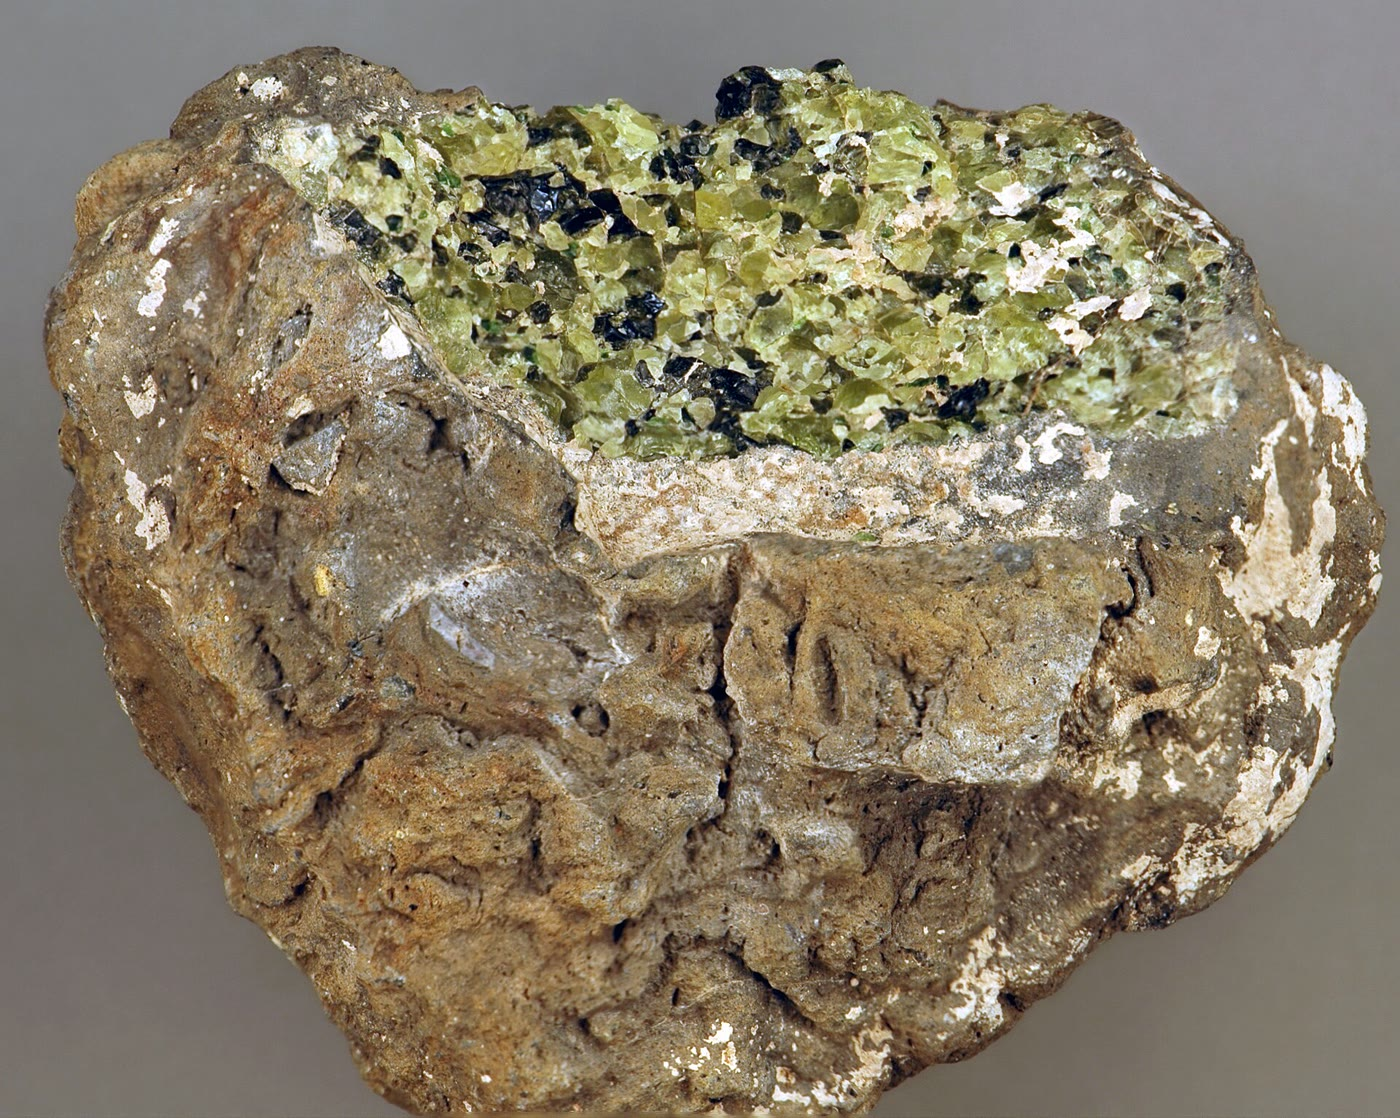
\includegraphics[width=\linewidth]{images/book4/b2-lherzolite-xenolith.jpg}
\end{minipage}\hfill
\begin{minipage}{0.48\linewidth}
{\small عقدة من بيريدوتيت الوشاح (لرزوليت) في حمم بازلتية من
كيلبورن هول، نيو مكسيكو، يبلغ عرضها \qty{7.4}{cm} في أعرض موضع: أوليفين
أصفر مخضرّ مع بيروكسين داكن. انتزعتها الحمم من الوشاح العلوي وحملتها
إلى السطح. James St.~John, CC BY 2.0.}
\end{minipage}
\end{omfigure}

يقارن الشكل أدناه هذه الأرض السيليكاتية بكوندريتات CI، عنصرًا
عنصرًا، بدلالة \omterm{def:b2:planet-formation-meteorites:condensation}{درجة حرارة التكاثف} التي قدّمها الفصل السابق. وهو يفرز
العناصر على نحو لا يستطيعه أي دليل آخر. فالعناصر المحبّة للصخور العصيّة على التبخّر،
من الزركونيوم \omterm{def:b2:elements-in-the-earth:ree}{والعناصر الأرضية النادرة} نزولًا إلى السترونشيوم والباريوم، تقف كلها
عند المستوى نفسه، في حدود عشرين في المئة بعضها من بعض: فقد احتفظت الأرض السيليكاتية
بها كلها بنسبها الكوندريتية. أمّا العناصر المحبّة للصخور المتطايرة
فتهبط مع درجة حرارة تكاثفها: إذ يوجد نحو خُمس البوتاسيوم
والصوديوم، وعُشر الروبيديوم، وجزء من مئة من الكلور، وبضعة
أجزاء من ألف من البروم واليود. والعناصر المحبّة للحديد تقع تحت كل عنصر محبّ للصخور
له التطاير نفسه بكثير: فالأرض السيليكاتية تحوي سُبع حصّتها من
الحديد، وجزءًا من ثلاثة عشر من النيكل، ونحو ثلاثة أجزاء من ألف من
فلزات مجموعة البلاتين والذهب. فقد ذهبت هذه إلى النواة. أمّا العناصر المحبّة
للكبريتيد، ومعظمها متطاير أيضًا، فمستنزفة من الوجهين.

\begin{omfigure}
\centering
\begin{tikzpicture}
\begin{axis}[omrecord, width=0.95\linewidth, height=8.2cm, ymode=log,
  xmin=500, xmax=1800, ymin=8e-4, ymax=3, x dir=reverse,
  xlabel={\foreignlanguage{arabic}{درجة حرارة التكاثف عند 50 في المئة تحت \babelsublr{\qty{e-4}{bar}} \babelsublr{(\unit{K})}}},
  ylabel={$(X/\mathrm{Mg})_{\mathrm{BSE}}\,/\,(X/\mathrm{Mg})_{\mathrm{CI}}$},
  legend pos=south west, legend cell align=left, legend style={font=\scriptsize},
  tick label style={font=\scriptsize}, label style={font=\small},
  scaled x ticks=false, xticklabel style={/pgf/number format/1000 sep={}}]
\addplot[black!40, dashed, domain=500:1800, samples=2, forget plot] {1};
\addplot[only marks, mark=*, mark size=1.6pt, brown!70!black]
  table[x=T, y=ratio] {figdata/out/bachelor-2-geochem-volat-lith.dat};
\addlegendentry{محبّة للصخور}
\addplot[only marks, mark=square*, mark size=1.6pt, blue!60!black]
  table[x=T, y=ratio] {figdata/out/bachelor-2-geochem-volat-sid.dat};
\addlegendentry{محبّة للحديد}
\addplot[only marks, mark=triangle*, mark size=2pt, orange!80!black]
  table[x=T, y=ratio] {figdata/out/bachelor-2-geochem-volat-chal.dat};
\addlegendentry{محبّة للكبريتيد}
\node[font=\tiny, brown!50!black, anchor=south] at (axis cs:1600,1.35)
  {\foreignlanguage{arabic}{\mbox{\textdir TLT Zr, Hf, Al, Sc, Y, Th, U, Ti, Ca, Sr, Ba} والعناصر الأرضية النادرة}};
\begin{scope}[font=\tiny, brown!50!black]
\node[anchor=west] at (axis cs:1328,1.0) {Mg};
\node[anchor=north] at (axis cs:1310,0.80) {Si};
\node[anchor=west] at (axis cs:1150,0.23) {Mn};
\node[anchor=south] at (axis cs:1142,0.47) {Li};
\node[anchor=south] at (axis cs:1010,0.195) {K};
\node[anchor=north] at (axis cs:958,0.22) {Na};
\node[anchor=north] at (axis cs:908,0.175) {B};
\node[anchor=north] at (axis cs:800,0.116) {Rb};
\node[anchor=south] at (axis cs:734,0.175) {F};
\node[anchor=west] at (axis cs:795,0.0477) {Cs};
\node[anchor=west] at (axis cs:944,0.0102) {Cl};
\node[anchor=north] at (axis cs:546,0.0061) {Br};
\node[anchor=south] at (axis cs:535,0.0088) {I};
\end{scope}
\begin{scope}[font=\tiny, blue!50!black]
\node[anchor=west] at (axis cs:1325,0.144) {Fe};
\node[anchor=east] at (axis cs:1364,0.0775) {Ni};
\node[anchor=west] at (axis cs:1342,0.088) {Co};
\node[anchor=west] at (axis cs:1780,0.137) {W};
\node[anchor=south] at (axis cs:1590,0.0206) {Mo};
\node[anchor=north] at (axis cs:883,0.0139) {Ge};
\node[anchor=north] at (axis cs:1500,0.0026) {Re, Os, Ir, Ru, Pt, Pd};
\node[anchor=north] at (axis cs:1060,0.0026) {Au};
\end{scope}
\begin{scope}[font=\tiny, orange!60!black]
\node[anchor=west] at (axis cs:1030,0.0993) {Cu};
\node[anchor=north] at (axis cs:996,0.0167) {Ag};
\node[anchor=south] at (axis cs:726,0.0746) {Zn};
\node[anchor=south] at (axis cs:704,0.0325) {Sn};
\node[anchor=east] at (axis cs:735,0.0246) {Pb};
\node[anchor=west] at (axis cs:648,0.0249) {Cd};
\node[anchor=east] at (axis cs:715,0.0022) {Te};
\node[anchor=north] at (axis cs:690,0.0016) {Se};
\node[anchor=west] at (axis cs:660,0.0019) {S};
\end{scope}
\end{axis}
\end{tikzpicture}
\par\smallskip{\small الأرض السيليكاتية مقارنةً بكوندريتات CI: لكل عنصر $X$، النسبة
$X/\mathrm{Mg}$ في \omterm{def:b2:elements-in-the-earth:bse}{الأرض السيليكاتية الكلية} مقسومةً على النسبة نفسها في كوندريتات
CI، بدلالة \omterm{def:b2:planet-formation-meteorites:condensation}{درجة حرارة التكاثف} عند 50 في المئة (الحارّ على اليسار).
العناصر المحبّة للصخور العصيّة على التبخّر كوندريتية بعضها نسبةً إلى بعض؛ والمتطايرة
مستنزفة مع انخفاض \omterm{def:b2:planet-formation-meteorites:condensation}{درجة حرارة التكاثف}؛ والعناصر المحبّة للحديد والمحبّة
للكبريتيد مستنزفة أكثر بكثير. البيانات: ماكدونو وصن (1995)؛
لودرز (2003).}
\end{omfigure}
% ledger: ms95:pm-trace, lodders:ci-table, lodders:tc-table, lodders:tc-more

تقف العناصر المحبّة للصخور العصيّة على التبخّر أعلى من المغنيسيوم بنحو 15 في المئة. ولا يمكن
للاثنين أن يكونا كوندريتيين تمامًا معًا: فإمّا أن الأرض اكتسبت \omterm{def:b2:elements-in-the-earth:volatility}{عناصر عصيّة}،
وإمّا أنها فقدت قليلًا من المغنيسيوم، وإمّا أن مغنيسيوم النموذج
مقدّر بأقل من حقيقته (\cref{exo:b2:elements-in-the-earth:12}). أمّا السيليكون، عند 0.83، فيقصر أكثر عن
المستوى العصيّ؛ وقد يكون جزء من السيليكون المفقود في النواة (المسألة).

إن العناصر المحبّة للحديد في الأرض السيليكاتية، مقرونةً بأرض كلية كوندريتية،
تزن النواة. لنفترض أن للأرض الكلية النسبة $r_X = X/\mathrm{Mg}$ التي في \omterm{def:b2:elements-in-the-earth:ci}{كوندريت CI}
لعنصر محبّ للحديد $X$، وأن النواة تحوي منه التركيز $c_X$
ولا تحوي مغنيسيومًا.

\begin{proposition}[الكسر الكتلي للنواة من نسبة كوندريتية]
\label{prop:b2:elements-in-the-earth:core}
لتكن $x$ الكسر الكتلي للنواة، و$C_X$ و$C_{\mathrm{Mg}}$
تركيزي $X$ والمغنيسيوم في الأرض السيليكاتية، و$c_X$ تركيز $X$ في
النواة. إذا كانت للأرض النسبة الكوندريتية $r_X$، فإن
\[
  \frac{x}{1-x} = \frac{r_X C_{\mathrm{Mg}} - C_X}{c_X}.
\]
\end{proposition}

\begin{proof}
تحوي كتلة $M$ من الأرض $(1-x)MC_X + xMc_X$ من $X$ و$(1-x)MC_{\mathrm{Mg}}$ من
المغنيسيوم. ونسبتهما هي $r_X$:
$(1-x)C_X + xc_X = r_X(1-x)C_{\mathrm{Mg}}$. والقسمة على $(1-x)c_X$ تعطي
النتيجة.
\end{proof}

مع الحديد، حيث $r_{\mathrm{Fe}} = \num{182800}/\num{95870} = 1.907$ في كوندريتات CI،
و22.8 في المئة من المغنيسيوم و6.26 في المئة من الحديد في الأرض السيليكاتية، و85.5 في
المئة من الحديد في نواة نموذجية، تعطي القضية $x/(1-x) = 0.435$، أي نواة تمثّل 30
في المئة من كتلة الأرض. أمّا علم الزلازل، بتكامل كثافة
النموذج المرجعي للأرض، فيعطي 32.5 في المئة. والاتفاق في حدود العُشر
يدعم صورة أرض كوندريتية معظم حديدها في النواة؛
والفرق يقيس مقدار ابتعاد نسبة الحديد إلى المغنيسيوم في الأرض عن
النسبة الكوندريتية (المسألة). والموازنة نفسها تبيّن أين يوجد كل عنصر من عناصر الأرض
(الشكل أدناه): فكل البلاتين والإيريديوم والذهب تقريبًا، ومعظم الحديد
والنيكل والكبريت، في النواة.
% ledger: lodders:ci-table, ms95:pm-trace, mcd03:core, data:prem

\begin{omfigure}
\centering
\begin{tikzpicture}
\begin{axis}[omrecord, xbar, width=0.8\linewidth, height=6.4cm, bar width=5pt,
  xmin=0, xmax=100, ymin=0.4, ymax=14.6, y dir=reverse,
  ytick={1,...,14}, yticklabels from table={figdata/out/bachelor-2-geochem-budget.dat}{el},
  xlabel={\foreignlanguage{arabic}{حصّة مخزون الأرض الموجودة في النواة (في المئة)}},
  tick label style={font=\scriptsize}, label style={font=\small},
  nodes near coords, nodes near coords align={horizontal},
  every node near coord/.append style={font=\tiny, /pgf/number format/fixed,
    /pgf/number format/precision=1}]
\addplot[fill=blue!35!gray!50, draw=black!60]
  table[x=share, y=idx] {figdata/out/bachelor-2-geochem-budget.dat};
\end{axis}
\end{tikzpicture}
\par\smallskip{\small أين توجد عناصر الأرض: حصّة كل عنصر الموجودة في
النواة، انطلاقًا من تركيب نموذجي للنواة، \omterm{def:b2:elements-in-the-earth:bse}{والوشاح البدائي}، ونواة تمثّل 32.5
في المئة من كتلة الأرض. البيانات: ماكدونو (2003)؛ ماكدونو وصن (1995)؛
النموذج المرجعي للأرض.}
\end{omfigure}
% ledger: mcd03:core, ms95:pm-trace, data:prem

\section{الوشاح والقشرتان}

انقسمت الأرض السيليكاتية منذ تكوّنها إلى وشاح ونوعين
من القشرة. فالقشرة المحيطية تُصنع بانصهار الوشاح تحت
الظهرات وسط المحيطية؛ والقشرة القارية بتاريخ طويل من الانصهار فوق
مناطق الاندساس، وإعادة التشكيل والتعرية (فصول لاحقة). ويرتكز النقاش على مصهورين
مرجعيين للوشاح.

\begin{definition}[بازلت الظهرات وسط المحيطية، بازلت الجزر المحيطية]
\label{def:b2:elements-in-the-earth:morb-oib}
\emph{بازلت الظهرات وسط المحيطية}\index{بازلت الظهرات وسط المحيطية} (MORB) بازلت
ينبثق عند ظهرة وسط محيطية، وهو صخر أعلى القشرة المحيطية.
و\emph{بازلت الجزر المحيطية}\index{بازلت الجزر المحيطية} (OIB) بازلت ينبثق
عند بركان محيطي بعيد عن حدود الصفائح، مثل براكين هاواي،
ويُعزى عادةً إلى عمود وشاحي (مجلد السنة الأولى).
\end{definition}

بازلت MORB المتوسط في الجدول أدناه متوسط عالمي بُني من 771 قطعة من
الظهرات، رُجّحت كل قطعة بطولها وبمعدل انفراجها، كي
يمثّل المتوسط القشرة التي تنتجها الظهرات. أمّا عمود
OIB فصخر واحد: المادة المرجعية البازلتية BHVO-2، المأخوذة عام 1995
من حمم فاضت من فوهة هاليماوماو في بركان كيلاويا، هاواي، عام 1919،
والتي حلّلتها مختبرات كثيرة، حتى إن معظم عناصرها الأرضية النادرة معروف بدقة
نحو واحد في المئة. والقشرة القارية العلوية متوسط مقدّر من
صخور السطح والرسوبيات.
% ledger: gale13:allmorb, usgs:bhvo2-origin, usgs:bhvo2-major, rg14:crust

\begin{table}[h]
\centering
\small
\begin{tabular}{lrrrr}
\hline
الأكسيد (\% كتلةً) & \omterm{def:b2:elements-in-the-earth:bse}{الوشاح البدائي} & MORB & \mbox{\textdir TLT OIB (BHVO-2)} & القشرة القارية العلوية\\
\hline
\ce{SiO2} & 45.0 & 50.47 & 49.60 & 66.6\\
\ce{TiO2} & 0.201 & 1.68 & 2.731 & 0.64\\
\ce{Al2O3} & 4.45 & 14.70 & 13.44 & 15.4\\
FeO (الكلي) & 8.05 & 10.43 & 11.15 & 5.04\\
MnO & 0.135 & 0.184 & 0.1690 & 0.10\\
MgO & 37.8 & 7.58 & 7.257 & 2.48\\
CaO & 3.55 & 11.39 & 11.40 & 3.59\\
\ce{Na2O} & 0.36 & 2.79 & 2.219 & 3.27\\
\ce{K2O} & 0.029 & 0.160 & 0.5130 & 2.80\\
\ce{P2O5} & 0.021 & 0.184 & 0.2685 & 0.15\\
\hline
\end{tabular}
\caption{تراكيب العناصر الرئيسية في أربعة خزّانات. تعطي BHVO-2 حديدها في صورة
\ce{Fe2O3} (12.39 في المئة)، وقد حُوّل هنا إلى FeO. البيانات: ماكدونو وصن
(1995)؛ غيل وآخرون (2013)؛ نشرة معلومات هيئة المسح الجيولوجي الأمريكية عن BHVO-2؛ رودنيك
وغاو (2014).}
\label{tab:b2:elements-in-the-earth:majors}
\end{table}
% ledger: ms95:pm-oxides, gale13:allmorb, usgs:bhvo2-major, rg14:crust

إذا قُرئ الجدول أفقيًا روى قصة الانصهار. فالوشاح بيريدوتيت غني
بالمغنيسيوم، فيه نحو 38 في المئة من MgO وأقل من 5 في المئة من \ce{Al2O3} وCaO.
ومصاهيره، أي البازلتات، تحوي مغنيسيومًا أقل بخمس مرات وكالسيومًا وألومنيومًا
أكثر بثلاث مرات: فالعناصر التي تدخل المصهور بسهولة تغادر الوشاح
أولًا. والبوتاسيوم والصوديوم والتيتانيوم أغنى أيضًا في المصاهير مقارنةً
بالوشاح، والبوتاسيوم أغنى ما يكون في القشرة القارية،
إذ يبلغ تركيزه فيها نحو مئة ضعف تركيزه في \omterm{def:b2:elements-in-the-earth:bse}{الوشاح البدائي}. ولا يرتفع السيليكون
من الوشاح إلى البازلتات إلا قليلًا، ويرتفع أكثر بكثير في القشرة
القارية، التي يقارب متوسطها تركيب الغرانوديوريت.

\section{العناصر النزرة}

تمثّل عشرة أكاسيد نحو 99 في المئة من كل صخر في الجدول أعلاه. أمّا بقية العناصر،
الموجودة بأجزاء في المليون، فتتبع العمليات نفسها التي تتبعها العناصر الرئيسية، لكنها
أشدّ حساسية لها بكثير.

\begin{definition}[العنصر النزر]\label{def:b2:elements-in-the-earth:trace}
\emph{العنصر النزر}\index{العنصر النزر} في صخر عنصر يكون
تركيزه، اصطلاحًا، أقل من 0.1 في المئة كتلةً (\qty{1000}{ppm}).
ونادرًا ما تكوّن العناصر النزرة معادن خاصة بها؛ بل تحلّ محل العناصر
الرئيسية في مواقع الشبكات البلّورية.
\end{definition}

\omterm{def:b2:elements-in-the-earth:trace}{العنصر النزر} مخفّف إلى حدّ أن تركيزه نفسه لا يغيّر
البلّورات ولا المصهور: فيكون توزّعه بينها نسبة بسيطة،
مستقلة عن تركيزه على مدى واسع.

\begin{definition}[معامل التوزيع بين المعدن والمصهور؛ العناصر المتوافقة
وغير المتوافقة]\label{def:b2:elements-in-the-earth:partition}
\emph{معامل التوزيع بين المعدن والمصهور}\index{معامل التوزيع بين المعدن والمصهور}
لعنصر في معدن هو نسبة تركيزيه في
المعدن وفي مصهور سيليكاتي متوازن معه،
$D = C_{\mathrm{mineral}}/C_{\mathrm{melt}}$. ومن أجل صخر من عدة معادن
كسورها الكتلية $x_i$، يكون \emph{معامل التوزيع الكلي}
$\bar D = C_{\mathrm{rock}}/C_{\mathrm{melt}}$. ويكون العنصر
\emph{عنصرًا متوافقًا}\index{العنصر المتوافق} في صخر إذا كان $\bar D > 1$،
و\emph{عنصرًا غير متوافق}\index{العنصر غير المتوافق} إذا كان $\bar D < 1$.
\end{definition}

\begin{proposition}[معامل التوزيع الكلي]
\label{prop:b2:elements-in-the-earth:bulk-d}
إذا كان كل معدن من معادن الصخر متوازنًا مع المصهور نفسه، فإن معامل التوزيع
الكلي هو متوسط معاملات المعادن مرجّحًا
بالكسور الكتلية: $\bar D = \sum_i x_i D_i$.
\end{proposition}

\begin{proof}
يحوي الصخر $C_{\mathrm{rock}} = \sum_i x_i C_i$، ويحوي كل معدن
$C_i = D_i C_{\mathrm{melt}}$. والقسمة على $C_{\mathrm{melt}}$ تعطي النتيجة.
\end{proof}

يتوقّف ملاءمة أيون لموقع على نصف قطره وشحنته. فالأيون القريب في
نصف قطره وشحنته من الأيون الرئيسي لموقع ما، مثل \ce{Ni^2+} مكان \ce{Mg^2+} في
الأوليفين، يدخل بسهولة ويكون متوافقًا. أمّا الأيون الأكبر بكثير، مثل
\ce{Rb+} أو \ce{Ba^2+}، أو الأعلى شحنةً، مثل \ce{Zr^4+} أو
\ce{Nb^5+}، فيُجهد الشبكة ويُطرد إلى المصهور: فهو
غير متوافق في معادن الوشاح. وتسلك مجموعتان من العناصر غير المتوافقة
سلوكين مختلفين لاحقًا، حين يتدخّل الماء.

\begin{definition}[العناصر المحبّة للصخور ذات الأيونات الكبيرة والعناصر ذات شدّة المجال العالية]
\label{def:b2:elements-in-the-earth:lile-hfse}
\emph{العناصر المحبّة للصخور ذات الأيونات الكبيرة}\index{العنصر المحبّ للصخور ذو الأيون الكبير}
(LILE) عناصر غير متوافقة أيوناتها كبيرة ضعيفة الشحنة، $+1$ أو $+2$:
البوتاسيوم والروبيديوم والسيزيوم والسترونشيوم والباريوم.
و\emph{العناصر ذات شدّة المجال العالية}\index{العنصر ذو شدّة المجال العالية} (HFSE)
عناصر غير متوافقة أيوناتها صغيرة عالية الشحنة، $+4$ أو $+5$:
الزركونيوم والهافنيوم والنيوبيوم والتنتالوم والتيتانيوم.
\end{definition}

تذوب العناصر LILE بسهولة في الموائع الغنية بالماء، ولا تكاد العناصر HFSE تذوب فيها. فالصخر
الذي غيّره الماء أو المصهور الذي ورث موائع، كما فوق مناطق الاندساس،
يحمل إذن عناصر LILE مع قليل من عناصر HFSE.

\begin{definition}[العناصر الأرضية النادرة]\label{def:b2:elements-in-the-earth:ree}
\emph{العناصر الأرضية النادرة}\index{العناصر الأرضية النادرة} (REE) هي اللانثانيدات
الخمسة عشر، من اللانثانوم إلى اللوتيتيوم؛ والبروميثيوم لا نظير مستقرًا له. وكلها
محبّة للصخور وعصيّة على التبخّر، وكلها تقريبًا ثلاثية التكافؤ، ونصف قطرها الأيوني
يتناقص بانتظام من اللانثانوم إلى اللوتيتيوم؛ ويمكن لليوروبيوم أن يكون ثنائي التكافؤ أيضًا في
المصاهير المختزَلة.
\end{definition}

لأن \omterm{def:b2:elements-in-the-earth:ree}{العناصر الأرضية النادرة} تختلف اختلافًا سلسًا في نصف القطر ولا شيء غيره،
فإنها تتجزّأ تجزّؤًا سلسًا: فالخفيفة منها، من اللانثانوم إلى الساماريوم، هي الأقل
توافقًا؛ والثقيلة، من الغادولينيوم إلى اللوتيتيوم، تلائم بعض
المعادن أكثر، ولا سيما الغارنت (الشكل أدناه). ففي صخر فيه غارنت تصير \omterm{def:b2:elements-in-the-earth:ree}{العناصر الأرضية النادرة}
الثقيلة متوافقة: فيكون مصهور مثل هذا الصخر غنيًا \omterm{def:b2:elements-in-the-earth:ree}{بالعناصر الأرضية النادرة} الخفيفة
وفقيرًا بالثقيلة.

\begin{omfigure}
\centering
\begin{tikzpicture}
\begin{axis}[omrecord, width=0.78\linewidth, height=6.4cm, ymode=log,
  xmin=0.6, xmax=9.4, ymin=5e-4, ymax=20,
  xtick={1,...,9}, xticklabels from table={figdata/out/bachelor-2-geochem-dvals.dat}{el},
  ylabel={\foreignlanguage{arabic}{معامل التوزيع $D$}}, legend pos=south east,
  legend cell align=left, legend style={font=\scriptsize},
  tick label style={font=\scriptsize}, label style={font=\small}]
\addplot[black!40, dashed, domain=0.6:9.4, samples=2, forget plot] {1};
\addplot[thick, green!45!black, mark=*] table[x=idx, y=cpx] {figdata/out/bachelor-2-geochem-dvals.dat};
\addlegendentry{كلينوبيروكسين}
\addplot[thick, red!70!black, mark=square*] table[x=idx, y=gar] {figdata/out/bachelor-2-geochem-dvals.dat};
\addlegendentry{غارنت}
\addplot[thick, olive!70!black, mark=triangle*] table[x=idx, y=ol] {figdata/out/bachelor-2-geochem-dvals.dat};
\addlegendentry{أوليفين + أورثوبيروكسين + سبينل}
\addplot[very thick, black, mark=diamond*] table[x=idx, y=bulk] {figdata/out/bachelor-2-geochem-dvals.dat};
\addlegendentry{\foreignlanguage{arabic}{الصخر الكلي (65/18/17 في المئة)}}
\node[font=\scriptsize, anchor=south west] at (axis cs:0.7,1) {متوافق};
\node[font=\scriptsize, anchor=north west] at (axis cs:0.7,1) {غير متوافق};
\end{axis}
\end{tikzpicture}
\par\smallskip{\small معاملات التوزيع بين المعدن والمصهور للعناصر الأرضية النادرة في
الكلينوبيروكسين والغارنت وخليط من الأوليفين والأورثوبيروكسين والسبينل، والمعامل
الكلي لبيروكسينيت غارنتي فيه 65 في المئة من الكلينوبيروكسين و18 في
المئة من الغارنت و17 في المئة من المعادن الأخرى (القضية أعلاه). يجعل الغارنت
\omterm{def:b2:elements-in-the-earth:ree}{العناصر الأرضية النادرة} الثقيلة متوافقة. البيانات: بودان (1991).}
\end{omfigure}
% ledger: budahn91:d-ree, budahn91:modes

\section{المخطّطات المُعايَرة}

تختلف وفرات العناصر المتجاورة بعوامل كبيرة بسبب التاريخ
النووي للمادة: فالعناصر ذات العدد الذرّي الزوجي أوفر من
جاراتها الفردية، كما يبيّن عمود CI للعناصر الأرضية النادرة (اللانثانوم 0.232،
والسيريوم 0.621، والبراسيوديميوم 0.0928 جزء في المليون). فإذا رُسمت \omterm{def:b2:elements-in-the-earth:ree}{العناصر الأرضية النادرة} لصخر كما هي شكّلت
خطًّا مسنّنًا يخفي تاريخه الجيولوجي. والقسمة على مرجع تزيله.
% ledger: lodders:ci-table

\begin{definition}[المخطّط المُعايَر]\label{def:b2:elements-in-the-earth:normalised}
\emph{المخطّط المُعايَر}\index{المخطّط المُعايَر} يرسم، لسلسلة من
العناصر بترتيب ثابت، التركيز في عيّنة مقسومًا على تركيزه في
مرجع، $X_N = C_X/C_X^{\mathrm{ref}}$، على مقياس لوغاريتمي. وتُعايَر \omterm{def:b2:elements-in-the-earth:ree}{العناصر الأرضية النادرة}
على كوندريتات CI بترتيب العدد الذرّي؛ أمّا مجموعة أطول من
العناصر غير المتوافقة، تسمّى غالبًا المخطّط العنكبوتي، فتُعايَر على
\omterm{def:b2:elements-in-the-earth:bse}{الوشاح البدائي} وتُرتّب حسب تناقص عدم توافقها في انصهار الوشاح.
\end{definition}

العيّنة التي لها نسب المرجع نفسها تُرسم خطًّا أفقيًا؛
وارتفاعه يعطي الإثراء. والميل يدلّ على تجزّؤ بين العناصر الخفيفة
والثقيلة، يُقاس بنسبة مثل $(\mathrm{La}/\mathrm{Yb})_N$. والعنصر
الوحيد الخارج عن الخط شذوذ.

\begin{proposition}[شذوذ اليوروبيوم]\label{prop:b2:elements-in-the-earth:normalised}
على \omterm{def:b2:elements-in-the-earth:normalised}{مخطّط مُعايَر} يكون فيه النمط خطًّا مستقيمًا في
$\log X_N$ بين الساماريوم والغادولينيوم، تكون القيمة المتوقّعة لليوروبيوم، الذي
يقع في المنتصف، $\mathrm{Eu}^* = \sqrt{\mathrm{Sm}_N\,\mathrm{Gd}_N}$.
و\emph{شذوذ اليوروبيوم}\index{شذوذ اليوروبيوم} هو
$\mathrm{Eu}/\mathrm{Eu}^* = \mathrm{Eu}_N/\sqrt{\mathrm{Sm}_N\,\mathrm{Gd}_N}$:
فهو سالب تحت 1، وموجب فوق 1.
\end{proposition}

\begin{proof}
الساماريوم واليوروبيوم والغادولينيوم متتالية بخطوات متساوية على المحور.
والخط المستقيم في $\log X_N$ يأخذ عند النقطة الوسطى متوسط القيمتين الطرفيتين:
$\log \mathrm{Eu}^* = \tfrac12(\log \mathrm{Sm}_N + \log \mathrm{Gd}_N)$، وهو
لوغاريتم المتوسط الهندسي.
\end{proof}

اليوروبيوم هو العنصر الأرضي النادر الوحيد الذي يمكن أن يكون ثنائي التكافؤ. وللأيون \ce{Eu^2+} تقريبًا
نصف قطر \ce{Ca^2+} و\ce{Sr^2+}، ولذلك يستقبله فلسبار البلاجيوكلاز حيث
يرفض \omterm{def:b2:elements-in-the-earth:ree}{العناصر الأرضية النادرة} الثلاثية التكافؤ. فالمصهور الذي تبلّر منه البلاجيوكلاز
ذو شذوذ سالب؛ والصخر الغني بالبلاجيوكلاز الباقي بعده ذو شذوذ موجب.

\begin{omfigure}
\centering
\begin{tikzpicture}
\begin{axis}[omrecord, width=0.8\linewidth, height=6.4cm, ymode=log,
  xmin=0.6, xmax=13.4, ymin=5, ymax=250,
  xtick={1,...,13}, xticklabels from table={figdata/out/bachelor-2-geochem-ree.dat}{el},
  ylabel={\foreignlanguage{arabic}{العيّنة / كوندريت CI}}, legend pos=north east, legend cell align=left,
  legend style={font=\scriptsize}, tick label style={font=\scriptsize},
  label style={font=\small}]
\addplot[thick, blue!70!black, mark=*] table[x=idx, y=morb] {figdata/out/bachelor-2-geochem-ree.dat};
\addlegendentry{\foreignlanguage{arabic}{متوسط MORB}}
\addplot[thick, red!70!black, mark=square*] table[x=idx, y=oib] {figdata/out/bachelor-2-geochem-ree.dat};
\addlegendentry{\foreignlanguage{arabic}{بازلت جزيرة محيطية (هاواي، BHVO-2)}}
\addplot[thick, brown!70!black, mark=triangle*] table[x=idx, y=ucc] {figdata/out/bachelor-2-geochem-ree.dat};
\addlegendentry{القشرة القارية العلوية}
\end{axis}
\end{tikzpicture}
\par\smallskip{\small أنماط \omterm{def:b2:elements-in-the-earth:ree}{العناصر الأرضية النادرة} مُعايَرةً على كوندريتات CI (حُذف الثوليوم
لعدم توفّر قيمة له في MORB). بازلت MORB المتوسط مستوٍ، أفقر قليلًا في \omterm{def:b2:elements-in-the-earth:ree}{العناصر الأرضية النادرة}
الخفيفة؛ والبازلت الهاوايي غني بها؛ والقشرة العلوية غنية بها بشدّة،
مع شذوذ سالب لليوروبيوم. البيانات: غيل وآخرون
(2013)؛ نشرة هيئة المسح الجيولوجي الأمريكية عن BHVO-2؛ رودنيك وغاو؛ لودرز (2003).}
\end{omfigure}
% ledger: gale13:allmorb, usgs:bhvo2-trace, rg03:ucc-trace, lodders:ci-table

تُقرأ الأنماط الثلاثة في الشكل أعلاه ثلاثة تواريخ. فبازلت MORB المتوسط
يقع أعلى من \omterm{def:b2:planet-formation-meteorites:chondrule}{الكوندريت} بنحو 25 مرة، مستويًا تقريبًا، مع $(\mathrm{La}/\mathrm{Sm})_N
= 0.85$: فقد فقد مصدره الوشاحي من قبلُ بعض أشدّ عناصره عدمَ توافق
لصالح مصاهير سابقة، ومنها القشرة القارية. والبازلت الهاوايي
غني \omterm{def:b2:elements-in-the-earth:ree}{بالعناصر الأرضية النادرة} الخفيفة، $(\mathrm{La}/\mathrm{Yb})_N = 5.4$، وعناصره
الأرضية النادرة الثقيلة أدنى من عناصر MORB: فقد جاء من درجة انصهار
أصغر، بقي فيها الغارنت محتفظًا بالثقيلة. والقشرة
القارية العلوية غنية باللانثانوم بأكثر من مئة مرة، مع
$(\mathrm{La}/\mathrm{Yb})_N = 10.9$ و$\mathrm{Eu}/\mathrm{Eu}^* = 0.72$: فهي
نتاج انصهار متكرّر، وعجز اليوروبيوم فيها يتّسق مع
بلاجيوكلاز بقي في القشرة العميقة.

\begin{omfigure}
\centering
\begin{tikzpicture}
\begin{axis}[omrecord, width=\linewidth, height=6.6cm, ymode=log,
  xmin=0.5, xmax=27.5, ymin=1, ymax=400,
  xtick={1,...,27}, xticklabels from table={figdata/out/bachelor-2-geochem-spider.dat}{el},
  ylabel={\foreignlanguage{arabic}{العيّنة / الوشاح البدائي}}, legend pos=north east, legend cell align=left,
  legend style={font=\scriptsize}, tick label style={font=\scriptsize},
  label style={font=\small}]
\addplot[thick, blue!70!black, mark=*, mark size=1.4pt] table[x=idx, y=morb] {figdata/out/bachelor-2-geochem-spider.dat};
\addlegendentry{\foreignlanguage{arabic}{متوسط MORB}}
\addplot[thick, red!70!black, mark=square*, mark size=1.4pt] table[x=idx, y=oib] {figdata/out/bachelor-2-geochem-spider.dat};
\addlegendentry{\foreignlanguage{arabic}{بازلت جزيرة محيطية (BHVO-2)}}
\addplot[thick, brown!70!black, mark=triangle*, mark size=1.6pt] table[x=idx, y=ucc] {figdata/out/bachelor-2-geochem-spider.dat};
\addlegendentry{القشرة القارية العلوية}
\end{axis}
\end{tikzpicture}
\par\smallskip{\small العناصر غير المتوافقة مُعايَرةً على \omterm{def:b2:elements-in-the-earth:bse}{الوشاح البدائي}، من الأشدّ
عدمَ توافق على اليسار. تُظهر القشرة القارية ارتفاع العناصر LILE، والقيعان
العميقة عند النيوبيوم والتنتالوم والتيتانيوم، وقمّة الرصاص الموروثة من
الانصهار في مناطق الاندساس؛ ويُظهر البازلت الهاوايي حدبة عند النيوبيوم
والتنتالوم. البوتاسيوم والتيتانيوم محسوبان من الأكاسيد. البيانات: كما في شكل \omterm{def:b2:elements-in-the-earth:ree}{العناصر
الأرضية النادرة}؛ ماكدونو وصن (1995).}
\end{omfigure}
% ledger: gale13:allmorb, usgs:bhvo2-trace, usgs:bhvo2-major, rg03:ucc-trace, ms95:pm-trace

يزيد المخطّط العنكبوتي أعلاه التباين حدّة. ففي القشرة القارية يقف
النيوبيوم والتنتالوم أدنى بكثير من جارَيهما الثوريوم واللانثانوم،
والتيتانيوم أدنى من جاريه، والرصاص أعلى بوضوح: $(\mathrm{Nb}/\mathrm{La})_N =
0.38$. وفي البازلت الهاوايي تبلغ النسبة نفسها 1.17، وفي بازلت MORB المتوسط
0.99. ونمط القشرة هو بصمة المصاهير فوق مناطق الاندساس، حيث
حملت الموائع العناصر LILE والرصاص إلى إسفين الوشاح وتركت العناصر HFSE وراءها
(فصول لاحقة)؛ وبازلتات الجزر المحيطية تخلو منه. ولذلك يمكن للمخطّط العنكبوتي لعيّنة واحدة
أن يميّز حمم قوس من حمم جزيرة محيطية، أو أن يكشف بازلتًا
ملوّثًا بالقشرة القارية (\cref{exo:b2:elements-in-the-earth:11}).

\begin{inthelab}[من صخر إلى قائمة عناصر نزرة]
\begin{minipage}[t]{0.6\linewidth}
\vspace{0pt}
يبدأ الجيوكيميائي الذي يريد العناصر النزرة لبازلت من بضع مئات من
الغرامات من أنقى أجزائه الداخلية، الخالية من القشرة المتجوّية ومن العروق. فيُسحق
الصخر، ثم يُطحن إلى مسحوق ناعم في طاحونة لا تلوّث مادتُها
العناصرَ المدروسة. ويُذاب جزء صغير من المسحوق
بالأحماض، أو يُصهر مع مُصهِر، ويُحلَّل المحلول بمطيافية
الكتلة ذات البلازما المقترنة حثّيًا، التي تقيس معظم
عناصر المخطّط العنكبوتي دفعة واحدة. ومع كل دفعة من العيّنات يحلّل
المختبر موادَّ مرجعية معلومة التركيب، مثل
البازلت الهاوايي BHVO-2: فقيمه آتية من دراسة جمعت متوسطات
مختبرات كثيرة، 132 منها للانثانوم، وبعضها، مثل قيمتي
النيوديميوم والساماريوم، بالتخفيف النظائري، الذي يعدّ ذرّات
عنصر مقابل كمية معلومة مضافة من أحد نظائره. فإذا وقعت نتيجة المختبر للمادة المرجعية
ضمن هامش عدم اليقين للقيمة المقبولة، قُبلت معها نتائج العيّنات
المجهولة.
\end{minipage}\hfill
\begin{minipage}[t]{0.36\linewidth}
\vspace{0pt}
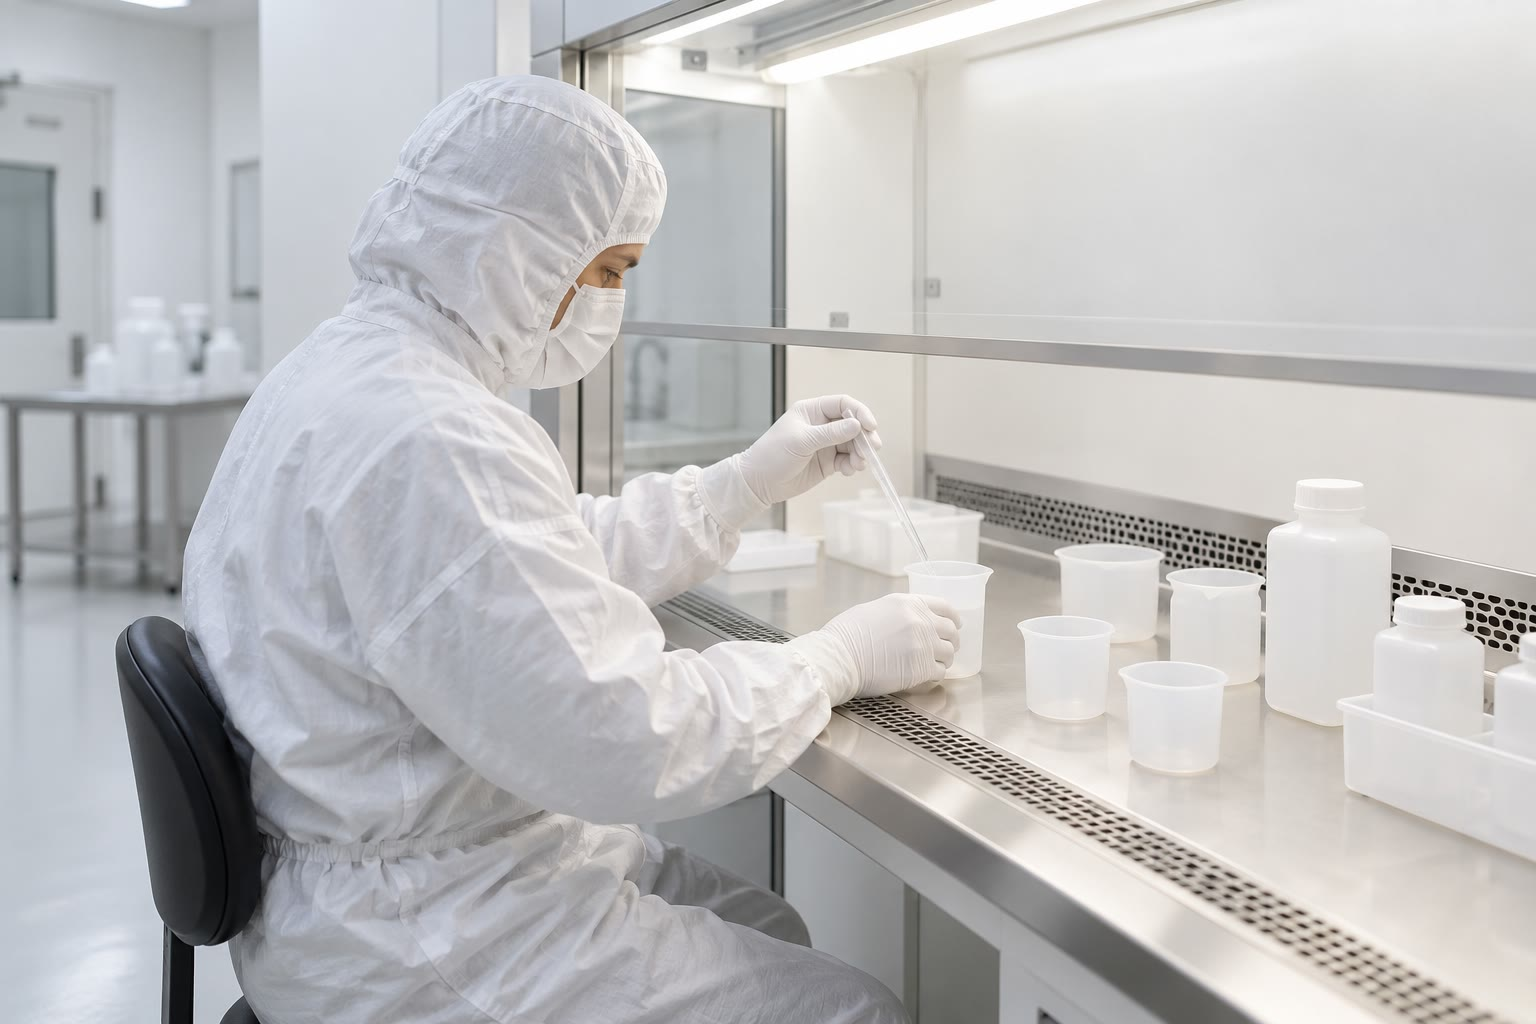
\includegraphics[width=\linewidth]{images/book4/ai/b2-clean-lab.jpg}

\smallskip
{\footnotesize عامل ببذلة الغرفة النظيفة عند منضدة التدفّق الصفائحي في
مختبر نظيف للجيوكيمياء (رسم توضيحي مولَّد بالذكاء الاصطناعي).\par}
\end{minipage}
\end{inthelab}
% ledger: usgs:bhvo2-trace, usgs:bhvo2-origin

\section{التمارين}

\begin{exercise}[$\star$]\label{exo:b2:elements-in-the-earth:1}
يحوي البازلت BHVO-2 كتلةً 0.5130 في المئة من \ce{K2O} و2.731 في المئة من \ce{TiO2}.
ومع الكتل الذرّية K 39.10 وTi 47.87 وO 16.00، احسب محتواه
من البوتاسيوم والتيتانيوم بالجزء في المليون.
\end{exercise}

\begin{exercise}[$\star$]\label{exo:b2:elements-in-the-earth:2}
في \omterm{def:b2:elements-in-the-earth:bse}{الأرض السيليكاتية الكلية}، تبلغ النسب $(X/\mathrm{Mg})$ مقسومةً على نسب CI
1.16 للألومنيوم، و0.22 للصوديوم، و0.077 للنيكل، و0.0029
للإيريديوم. ودرجات حرارة تكاثف هذه العناصر هي 1653 و958 و1353
و\qty{1603}{K}. اذكر صنف غولدشميت لكل عنصر وفسّر كل
استنزاف.
\end{exercise}

\begin{exercise}[$\star$]\label{exo:b2:elements-in-the-earth:3}
تحوي القشرة القارية العلوية \qty{31}{ppm} من اللانثانوم و\qty{2.0}{ppm}
من الإتربيوم؛ وتحوي كوندريتات CI منهما 0.232 و\qty{0.163}{ppm}. احسب
القيم المُعايَرة على \omterm{def:b2:planet-formation-meteorites:chondrule}{الكوندريت} و$(\mathrm{La}/\mathrm{Yb})_N$. ماذا تقول
النسبة عن القشرة؟
\end{exercise}

\begin{exercise}[$\star$]\label{exo:b2:elements-in-the-earth:4}
تحوي القشرة القارية العلوية 4.7 و1.0 و\qty{4.0}{ppm} من الساماريوم
واليوروبيوم والغادولينيوم؛ وكوندريتات CI منها 0.145 و0.0546 و\qty{0.198}{ppm}.
احسب $\mathrm{Eu}/\mathrm{Eu}^*$. أيّ معدن يفسّر النتيجة؟
\end{exercise}

\begin{exercise}[$\star\star$]\label{exo:b2:elements-in-the-earth:5}
يتكوّن بيروكسينيت غارنتي من 65 في المئة كلينوبيروكسين، و18 في المئة غارنت،
و17 في المئة أوليفين وأورثوبيروكسين وسبينل. ومعاملات توزيع
اللانثانوم 0.058 و0.001 و0.001، ومعاملات اللوتيتيوم 0.53 و5.8 و0.18.
احسب المعاملين الكليين. أيّ العنصرين متوافق في الصخر؟ وأيّ
معدن يحوي معظم لوتيتيوم الصخر؟
\end{exercise}

\begin{exercise}[$\star\star$]\label{exo:b2:elements-in-the-earth:6}
تحوي \omterm{def:b2:elements-in-the-earth:bse}{الأرض السيليكاتية الكلية} 22.8 في المئة من المغنيسيوم، و\qty{2670}{ppm} من
الصوديوم، و\qty{1960}{ppm} من النيكل؛ وتحوي كوندريتات CI منها 9.587 في المئة
و\qty{5010}{ppm} و\qty{10640}{ppm}. احسب النسب المُعايَرة على المغنيسيوم نسبةً إلى CI
للصوديوم والنيكل. كلا العنصرين يتكاثف قرب \qty{1000}{K} أو فوقها؛ فلماذا
النيكل هو الأشدّ استنزافًا؟
\end{exercise}

\begin{exercise}[$\star\star$]\label{exo:b2:elements-in-the-earth:7}
يتبلّر كلينوبيروكسين من مصهور له تركيب بازلت MORB المتوسط،
\qty{5.21}{ppm} من اللانثانوم و\qty{0.53}{ppm} من اللوتيتيوم. ومعاملا
توزيعه 0.058 للانثانوم و0.53 للوتيتيوم. احسب محتواه من
اللانثانوم واللوتيتيوم، ونسبة $(\mathrm{La}/\mathrm{Lu})_N$
في البلّورة إلى نظيرتها في المصهور (CI: La 0.232، Lu \qty{0.0237}{ppm}).
\end{exercise}

\begin{exercise}[$\star\star$]\label{exo:b2:elements-in-the-earth:8}
بالمعايرة على \omterm{def:b2:elements-in-the-earth:bse}{الوشاح البدائي} (Nb \qty{0.658}{ppm}، La \qty{0.648}{ppm})،
احسب $(\mathrm{Nb}/\mathrm{La})_N$ للقشرة القارية العلوية (Nb 12،
La \qty{31}{ppm})، وللبازلت الهاوايي (18.10، \qty{15.20}{ppm})، ولبازلت MORB المتوسط
(5.24، \qty{5.21}{ppm}). أيّها يحمل بصمة مناطق الاندساس؟
\end{exercise}

\begin{exercise}[$\star\star$]\label{exo:b2:elements-in-the-earth:9}
البوتاسيوم واليورانيوم كلاهما شديد عدم التوافق. احسب النسبة الكتلية K/U في
\omterm{def:b2:elements-in-the-earth:bse}{الوشاح البدائي} (K \qty{240}{ppm}، U \qty{0.0203}{ppm})، وفي بازلت MORB المتوسط
(\qty{0.160}{\percent} \ce{K2O}، U \qty{0.119}{ppm})، وفي القشرة القارية
العلوية (\qty{2.80}{\percent} \ce{K2O}، U \qty{2.7}{ppm})، مستعملًا
$\mathrm{K}/\ce{K2O} = 0.830$ كتلةً. ماذا يعني ثبات النسبة تقريبًا،
ولماذا تفيد K/U في تقدير بوتاسيوم كوكب؟
\end{exercise}

\begin{exercise}[$\star\star\star$]\label{exo:b2:elements-in-the-earth:10}
كمية صغيرة من المصهور متوازنة مع البيروكسينيت الغارنتي في التمرين
5. بيّن أنه، من أجل عنصرين، تساوي النسبة
$(C_1/C_2)_{\mathrm{melt}}/(C_1/C_2)_{\mathrm{rock}}$
$\bar D_2/\bar D_1$. احسبها للانثانوم واللوتيتيوم، وفسّر لماذا تكون
لمصاهير الوشاح الحامل للغارنت أنماط عناصر أرضية نادرة شديدة الانحدار.
\end{exercise}

\begin{exercise}[$\star\star\star$]\label{exo:b2:elements-in-the-earth:11}
يتمثّل بازلت MORB متوسط (Th \qty{0.404}{ppm}، Nb \qty{5.24}{ppm}) قشرةً قارية
علوية (Th \qty{10.5}{ppm}، Nb \qty{12}{ppm}): فيمتزج كسر كتلي $f$ من
القشرة مع $1-f$ من البازلت. بيّن أن تراكيز المزيج
خطية في $f$ لكن نسبته Th/Nb ليست كذلك. أوجد $f$ التي تبلغ عندها Th/Nb
0.2، والنسبة من أجل $f = 0.1$.
\end{exercise}

\begin{exercise}[$\star\star\star$]\label{exo:b2:elements-in-the-earth:12}
إزالة الماء أو الكربون أو نواة فلزية لا تحوي ألومنيومًا ولا
مغنيسيومًا لا تغيّر النسبة Al/Mg للباقي: بيّن ذلك. في \omterm{def:b2:elements-in-the-earth:bse}{الأرض السيليكاتية
الكلية} تبلغ $(\mathrm{Al}/\mathrm{Mg})$ 1.16 ضعف قيمة CI. إذا كانت
الأرض قد احتفظت بكل ألومنيومها، فما كسر مغنيسيومها الكوندريتي
المفقود من الأرض السيليكاتية؟ ومع النسبة المُعايَرة على المغنيسيوم للسيليكون،
0.83، ما كسر سيليكونها الكوندريتي الذي يكون مفقودًا بالافتراض
نفسه؟
\end{exercise}

\section{مسألة: وزن النواة بكوندريت}

\begin{problem}[{مسألة نهاية الأسبوع --- إعادة بناء الأرض الكلية من كوندريتات CI
والوشاح والنواة، ووزن النواة}]
\label{pb:b2:elements-in-the-earth:1}
تريد جيوكيميائية كوكبية أن تزن نواة الأرض دون علم الزلازل، من
الكيمياء وحدها. فتتّخذ كوندريتات CI مادةً ابتدائية (Mg
\qty{95870}{ppm}، Al 8500، Si \num{106500}، Fe \num{182800}، Ni
\qty{10640}{ppm})، \omterm{def:b2:elements-in-the-earth:bse}{والوشاح البدائي} للأرض السيليكاتية (MgO 37.8، FeO
8.05، NiO 0.25 في المئة؛ Mg 22.8، Si 21.0 في المئة)، ونواة نموذجية فيها 85.5
في المئة Fe و5.2 في المئة Ni و6.0 في المئة Si. الكتل الذرّية: Mg 24.31،
Si 28.09، Fe 55.85، Ni 58.69، O 16.00. كتلة الأرض
\qty{5.972e24}{kg}.

\medskip\noindent\textbf{الجزء الأول --- نقطة البداية الكوندريتية.}
\begin{enumerate}
\item احسب النسب الكتلية Fe/Mg وNi/Mg وSi/Mg وAl/Mg في كوندريتات CI.
\item حوّل Fe/Si إلى نسبة ذرّية. تعطي مطيافية الفوتوسفير الشمسي
0.81 ذرّة حديد لكل ذرّة سيليكون: هل المقارنة معقولة؟
\item تحوي كوندريتات CI 2.1 في المئة من الهيدروجين و3.5 في المئة من الكربون، مرتبطة في
معادن حاملة للماء ومركّبات عضوية لم تحتفظ بها الأرض. لماذا
لا تحتاج نسب السؤال 1 إلى تصحيح لهذا الفقد؟
\item لماذا يصلح المغنيسيوم عنصرًا مرجعيًا لمسألة النواة،
ولماذا لا يصلح الحديد؟
\item يتكاثف النيكل والمغنيسيوم والحديد والسيليكون في حدود \qty{50}{K} بعضها من
بعض (1353 و1336 و1334 و\qty{1310}{K}). لماذا يدعم هذا
افتراض أن الأرض الكلية احتفظت بنسبها الكوندريتية؟ وأيّ نسبة من
نسب السؤال 1 تشذّ عن هذه المجموعة، وماذا يقول الفصل عنها؟
\end{enumerate}

\noindent\textbf{الجزء الثاني --- الأرض السيليكاتية.}
\begin{enumerate}[resume]
\item حوّل FeO وNiO في \omterm{def:b2:elements-in-the-earth:bse}{الوشاح البدائي} إلى Fe وNi.
\item احسب Fe/Mg وNi/Mg في الأرض السيليكاتية.
\item ما كسر Fe وNi الكوندريتيين المفقود من الأرض
السيليكاتية، عند مغنيسيوم ثابت؟
\item الحساب نفسه للإيريديوم (\omterm{def:b2:elements-in-the-earth:bse}{الوشاح البدائي} \qty{3.2}{ppb}، CI
\qty{0.470}{ppm}) يعطي كسرًا مفقودًا قدره 99.7 في المئة. لماذا هو أكبر
منه للنيكل، وكسر النيكل أكبر منه للحديد؟
\item أين يوجد الحديد في الأرض السيليكاتية، ولماذا لم يذهب كله إلى
النواة؟
\end{enumerate}

\noindent\textbf{الجزء الثالث --- وزن النواة.}
\begin{enumerate}[resume]
\item اكتب موازنة الحديد في الأرض بدلالة الكسر الكتلي للنواة $x$،
واستنتج \cref{prop:b2:elements-in-the-earth:core}.
\item احسب $y = x/(1-x)$ و$x$ من الحديد.
\item افعل الشيء نفسه من النيكل.
\item التقديران لا يتّفقان تمامًا. اجمعهما بطريقة المربعات الصغرى:
اجعل $\sum (a_iy - b_i)^2$ أصغر ما يمكن، حيث $a_i y = b_i$ معادلتا
السؤالين 12 و13، وأعطِ أفضل $y$ و$x$.
\item لماذا تقع قيمة المربعات الصغرى قريبة جدًا من تقدير الحديد؟
\item من المعادلتين، احسب نسبة Fe/Ni في النواة التي تجعل
كلتيهما صحيحتين تمامًا. وقارن بالنواة النموذجية.
\item أعطِ كتلة النواة.
\end{enumerate}

\noindent\textbf{الجزء الرابع --- تحقّقات ونتائج.}
\begin{enumerate}[resume]
\item يعطي علم الزلازل نواة تمثّل 32.5 في المئة من كتلة الأرض. بكم في
المئة يختلف التقدير الكيميائي؟
\item مع نواة تمثّل 32.5 في المئة، كم من الحديد ينبغي أن تحوي النواة لكي
تُغلق موازنة الحديد؟ وهل يتوافق هذا مع نواة 10 في المئة منها عناصر
خفيفة؟
\item تحوي النواة النموذجية 9.3 في المئة من عناصر غير Fe وNi. ما العناصر
الخفيفة المرشّحة، وأيّ دليل في الفصل يدعم السيليكون؟
\item احسب، مع $y$ السؤال 14، محتوى النواة من السيليكون الذي
يجعل نسبة Si/Mg في الأرض الكلية كوندريتية.
\item قارن بالقيمة 6 في المئة في النموذج. واقترح سببًا، من الفصل
السابق، لكون بعض السيليكون قد يكون مفقودًا من الأرض كليًّا.
\item تحوي النواة النموذجية \qty{0.5}{ppm} من الذهب، \omterm{def:b2:elements-in-the-earth:bse}{والوشاح البدائي}
\qty{1}{ppb}. مع نواة تمثّل 32.5 في المئة، ما كسر ذهب الأرض الموجود
في النواة؟
\item اذكر الكسر الكتلي لنواة الأرض المستخلص من الكيمياء وحدها،
وهو الرقم الأساسي في هذه المسألة.
\end{enumerate}
\end{problem}
% ledger: lodders:ci-table, lodders:ci-h-photo, ms95:pm-oxides, ms95:pm-trace, mcd03:core, earth:mass, badro:core, lodders:tc-table
